\documentclass[10pt]{beamer}

\usetheme{Boadilla}

\usepackage{pgf}
\usepackage[english]{babel}
\usepackage[utf8]{inputenc}
\usepackage{epstopdf}

\usepackage{bm}
%\usepackage[opticals,mathlf,onlytext]{MinionPro}
\usepackage{mathpazo}
\usepackage[euler-digits,euler-hat-accent]{eulervm}

% graphics

\usepackage{tabularx}

\usepackage{subcaption}
\usepackage{rotating}
\usepackage{pgffor}
\usepackage{tikz}
\usepackage{ifthen}

\usepackage{graphicx}

\newcommand\myheader[1]{%
  \ifcase#1\relax invisible
  \or (a) \or (b) \or (c) \or (d) \or (e) \or (f) 
  \or (g) \or (h) \or (i) \or (j) \or (k) \or (l) 
  \or (m) \or (n) \or (o) \or (p) \or (q) \or (r) 
  \or (s) \or (t) \or (u) \or (v) \or (w) \or (x) 
  \or (y) \else (z)
  \fi
}

%\setbeamercolor{structure}{fg=Ma}

%\usepackage{times}
%\usepackage[T1]{fontenc}

%\usepackage{graphicx}
%\usepackage{epstopdf}
%\DeclareGraphicsExtensions{.pdf,.eps,.png,.jpg,.mps} 

\title[Defensa de Tesis] %
{Segmentaci\'on de interlocutores a partir de se\~nales de audio utilizando cadenas escondidas de Markov  y t\'ecnicas de selecci\'on autom\'atica de modelos}

%\subtitle{Include Only If Paper Has a Subtitle}

\author[Rafael de Jes\'us Robledo Ju\'arez]%
{Rafael de Jes\'us Robledo Ju\'arez \\
\small{\texttt{rrobledo@cimat.mx}} \\ ~\\
\small{Asesor: Dr. Salvador Ru\'iz Correa}}


\institute[CIMAT] % (optional, but mostly needed)
{
  \pgfuseimage{university-logo} ~ \\
  Centro de Investigaci\'on en Matem\'aticas, Guanajuato \\
  Departamento de Ciencias de la Computación
}

\date[noviembre 2013]
{xx de noviembre del 2013}
\subject{\title}

\pgfdeclareimage[interpolate=true, height=2cm]{university-logo}{logos/logo-big}
\pgfdeclareimage[interpolate=true, height=0.5cm]{department-logo}{logos/logo-trans}
%\logo{\pgfuseimage{department-logo}}
\logo{
	\pgfputat{\pgfxy(-0.3, 0)}{
    %\begin{pgfrotateby}{\pgfdegree{30}}
    %  \pgfbox[center,base]{\pgfuseimage{department-logo}}
    %\end{pgfrotateby}
	}
}

\AtBeginSection[] {
  \begin{frame}
   \frametitle{Contenido}
    \tableofcontents[currentsection, hideothersubsections]
    \addtocounter{framenumber}{-1}
  \end{frame}
}

\usecolortheme[RGB={79, 17, 32}]{structure} 
\setbeamercolor{alerted text}{use=structure,fg=structure!50!red}

\setbeamertemplate{navigation symbols}{} 

\def\mb{\textbf}
\def\mc{\mathcal}

\begin{document}
\setbeamertemplate{itemize items}[default]
\setbeamertemplate{enumerate items}[default]
\setbeamerfont{section number projected}{series=\bfseries,size={\fontsize{8}{12}}}
\setbeamertemplate{sections/subsections in toc}[square]

\begin{frame}
  \titlepage
\end{frame}


\begin{frame}{Contenido}
  \setcounter{tocdepth}{1}
  \tableofcontents
  \setcounter{tocdepth}{4}  
\end{frame}

%!TEX root = ../pres - final.tex

%\setlength{\itemsep}{3em}

\section{Introducción}

\subsection{Problema}
\begin{frame}{Problema}

\begin{itemize}
    \itemsep1em
    \item Se considera que se tiene una señal de audio con información de nuestro interés, y se requiere segmentar de acuerdo a las personas que participan en la grabación.

    \item \alert{\textit{Speaker Diarization}}: el problema consiste en identificar el número de interlocutores que participan en una grabación de audio, y además encontrar en qué segmentos de la grabación habla cada persona.

    \item Dos tareas principales: 
    \begin{enumerate}
        \item Encontrar el número total de personas que hablan en la conversación.
        \item Identificar los momentos en los que habla cada participante.
    \end{enumerate}
  \end{itemize}

\end{frame}

\subsection{Motivación}

\begin{frame}{Motivación}
  \begin{itemize}
    \itemsep1em
    \item  La tarea de speaker diarization es importante en diferentes procesos que se realizan con las grabaciones de audio, tales como la identificación y navegación por segmentos en específico.

    \item También resulta útil para la búsqueda y recuperación de información en grandes volúmenes de secuencias de audio.
  
    \item Es una etapa importante en el procesamiento de voz. Tanto para reconocimiento como transcripción de voz.
    
  \end{itemize}
\end{frame}

\subsection{Principales enfoques}
\begin{frame}{Principales enfoques}
  De acuerdo al trabajo desarrollado hasta ahora, se pueden distinguir dos grandes enfoques:
  
  \begin{description}
    \itemsep1.5em
    \item[\textit{Bottom-up:}]
      Se inicia la estimación con pocos clústers (e incluso un segmento único)
    \item[\textit{Top-down:}]
      Se inicia la estimación con muchos más grupos de los que se esperan encontrar.
  \end{description}

   Ambas metodologías iteran hasta converger a un número de clústers óptimo, en que cada grupo debe corresponder a un interlocutor.
\end{frame}    

\subsection{Trabajo previo}
\begin{frame}{Trabajo previo}
  You can create overlays\dots
  \begin{itemize}
  \item using the \texttt{pause} command:
    \begin{itemize}
    \item
      First item.
    \item    
      Second item.
    \end{itemize}
  \item
    using overlay specifications:
    \begin{itemize}
    \item
      First item.
    \item
      Second item.
    \end{itemize}
  \item
    using the general \texttt{uncover} command:
    \begin{itemize}
      \item
        First item.
      \item
        Second item.
    \end{itemize}
  \end{itemize}
\end{frame}

%!TEX root = ../pres - final.tex

\section{Speaker Diarization}

\subsection{Formulación matemática}
\begin{frame}{Formulación matemática (I)}
Denótese por $\mathcal{A}$ la evidencia acústica a partir de la cuál el modelo deberá encontrar la segmentación correcta para un fragmento de señal.
\\~\\
Se puede pensar en $\mathcal{A}$ como la secuencia de símbolos correspondiente a un segmento de señal, y que está conformada por elementos de un alfabeto mucho más grande $\mathbb{A}$. 
\begin{equation}
\mathcal{A} = a_1, a_2, ..., a_K \quad a_i \in \mathbb{A}
\label{eqn:2a-1}
\end{equation}
en donde los elementos $a_i$ hacen referencia a un intervalo de tiempo $i$ en la secuencia de audio original.
%, y los valores que tomen pueden repetirse de acuerdo a la grabación.
\vfill
De la misma manera,
\begin{equation}
\mathcal{S} = s_1, s_2, ..., s_N \quad s_i \in \mathbb{S}
\label{eqn:2a-2}
\end{equation}
donde $\mathcal{S}$ es la secuencia que corresponde a la segmentación correcta para un intervalo del audio original. 
\\~\\
$\mathbb{S}$ es el conjunto de todos los interlocutores que participan en la grabación de audio y $s_i$ de igual manera representa al interlocutor que habla en el tiempo $i$.
\end{frame}

\begin{frame}{Formulación matemática (II)}
Si $P(\mathcal{S} \,|\, \mathcal{A})$ es la probabilidad de que una secuencia de interlocutores $\mathcal{S}$ esté hablando dada la evidencia acústica en $\mathcal{A}$, entonces para escoger cuáles son los personas que hablan en ese intervalo se calcula:
\begin{equation}
\hat{\mathcal{S}} = \underset{\mathcal{S}}{arg~max}~ P(\mathcal{S} \,|\, \mathcal{A})
\label{eqn:2a-3}
\end{equation}
%Seleccionaría la sucesión de interlocutores más probable para una secuencia de datos dada.
%\\~\\
\vfill
Que por el Teorema de Bayes, es equivalente a maximizar: 
\begin{equation}
\hat{\mathcal{S}} = \underset{\mathcal{S}}{arg~max}~ P(\mathcal{S}) \cdot P(\mathcal{A} \,|\, \mathcal{S})
\label{eqn:2a-6}
\end{equation}
pues la variable $\mathcal{A}$ es constante respecto a $\mathcal{S}$. %-pues es la única evidencia acústica observada-

\end{frame}

\subsection{Componentes del sistema (I)}
\begin{frame}{Componentes del sistema}
  En general, todos los sistemas que involucran procesamiento de
  voz, tienen varias etapas esenciales, como se menciona en Jelinek (cita)

  \begin{enumerate}
    \itemsep1em
    \item \structure{Procesamiento acústico:}
    Se refiere a la forma en la que se procesará la información y se digitalizará.% Usualmente se contará con un micrófono o un arreglo de micrófonos que captarán las voces y las transformarán en impulsos eléctricos. 
    %\\~\\
    Además se debe realizar algún proceso para obtener una representación paramétrica de la señal. A este procedimiento se le conoce como construcción del \textit{diccionario de palabras}.

    \item \structure{Modelado acústico:}
    Se considera que ya se ha construido el diccionario de palabras o la evidencia acústica $\mathbb{A}$, y se necesita proponer una forma de calcular las probabilidades $P(\mathcal{A} \,|\, \mathcal{S})$. 
    % \\~\\
    El modelo acústico más comúnmente utilizado en tareas de procesamiento de voz, es el HMM, aunque hay trabajos que utilizan otras técnicas: ANN \cite{Jothilakshmi2009} \cite{Gutzwiller2010}  o métodos de DTW \cite{Huijbregts2011} 
  \end{enumerate}

\end{frame}

\begin{frame}{Componentes del sistema (II)}
  \begin{enumerate}
    \item \structure{Modelado de interlocutores:}
    \item \structure{Búsqueda de hipótesis:}
  \end{enumerate}

\end{frame}

\subsection{Procesamiento acústico}

\begin{frame}{Elminación de ruido / Detección de silencios}
  \begin{center}
    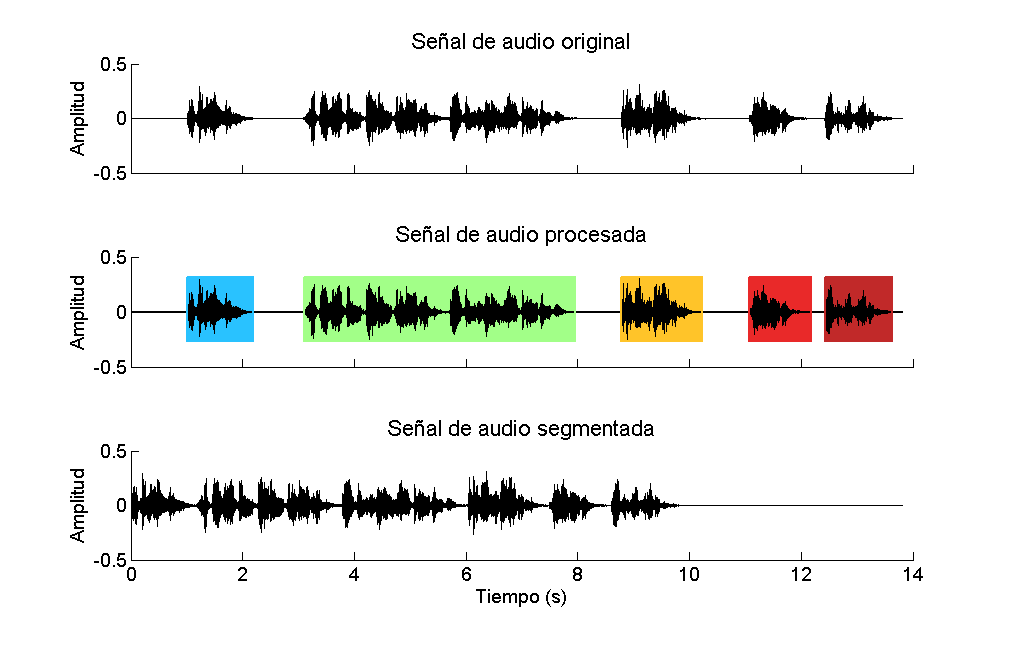
\includegraphics[width=1\textwidth]{gfx/f-silence}
  \end{center}
\end{frame}

%\subsubsection{Obtención de vector de características}

\begin{frame}{Mel Frequency Cepstrum Coefficient}
  \begin{itemize}
    \item \small{FFT (ventana) -> Banco de filtros triangular (Mel Scale) -> Log -> DCT -> MFCC}
  \end{itemize} 
  \begin{center}
    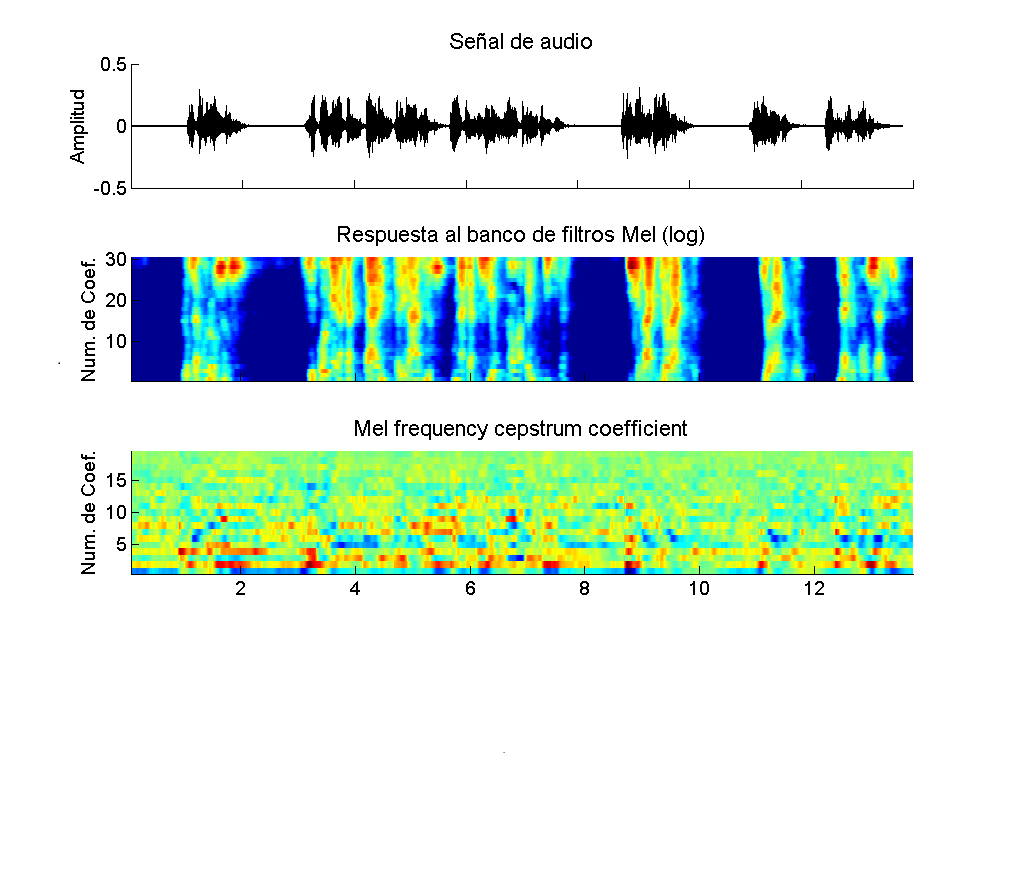
\includegraphics[width=1\textwidth]{gfx/f-mfcc}
  \end{center}
\end{frame}

%!TEX root = ../pres - final.tex

\section{Modelo}
\subsection{Hidden Markov Model}
\begin{frame}{Cadenas de Markov}
    \begin{itemize}
      \itemsep2em
      \item Cadena de Markov de primer orden      
        \\~\\
        \begin{center}
          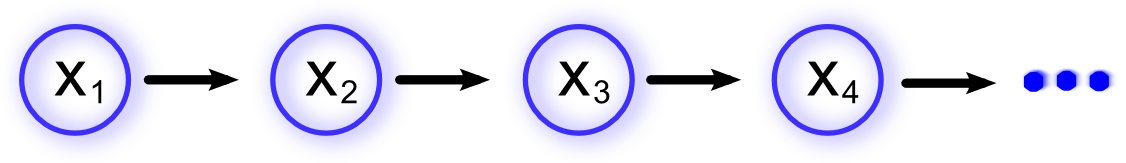
\includegraphics[width=0.4\textwidth]{gfx/mod-mm1}
        \end{center}        
        \begin{equation}
          \label{eqn:2-4}
          p(x_1, ..., x_T) 
            ~=~ \prod_{t=1}^T p(x_T ~|~ x_1, ..., x_{t-1}) 
            ~=~ p(x_1) \cdot \prod_{t=2}^T p(x_T ~|~ x_{t-1}) 
        \end{equation} 
      \item  Se puede generalizar para cadenas de Markov de un orden mayor
        \\~\\
        \begin{center}
          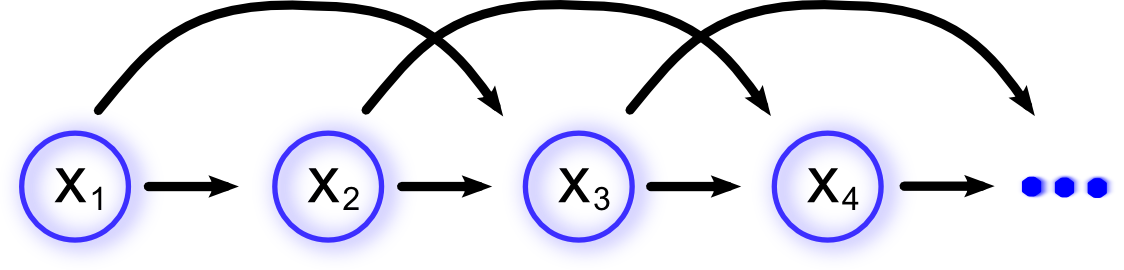
\includegraphics[width=0.45\textwidth]{gfx/mod-mm2}
        \end{center}
        \begin{equation}
          \label{eqn:2-4}
          p(x_1, ..., x_T) 
            ~=~ p(x_1) p(x_2 ~|~ x_1) \cdot \prod_{t=3}^T p(x_T ~|~ x_{t-1}, x_{t-2}) 
        \end{equation} 
  \end{itemize} 
\end{frame}

\begin{frame}{Modelo oculto de Markov}
  \begin{itemize}
    \itemsep1em
    \item Agregar una variable latente $z_t$ (discreta), que corresponda a cada observación $x_t$.
      \begin{align}
        z_{t+1} &\perp z_{t-1} ~|~ z_{t} \\
        p(x_1, ..., x_T, z_1, ..., z_T) &~=~ p(z_1) \left [ \prod_{t=2}^T p(z_t ~|~ z_{t-1}) \right ] 
          \prod_{t=1}^T p(x_t ~|~ z_{t}).
      \end{align}

    \item Modelar proceso bivariado en el tiempo. Una variable observada y una variable latente asociada.
      \\~\\
      \begin{center}
        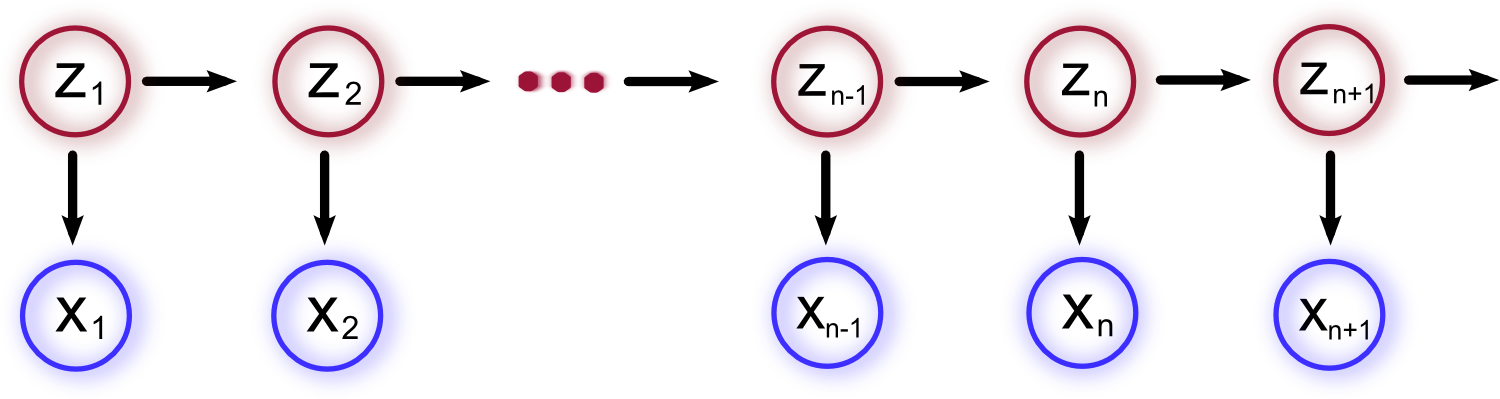
\includegraphics[width=0.5\textwidth]{gfx/mod-hmm}
      \end{center}    
      
    \item Mezcla de distribuciones en la que la densidad está dada por $p(x | z)$      
  \end{itemize}
\end{frame}

\begin{frame}{Parámetros del HMM}
  \begin{itemize}
    \item Probabilidad de cambio entre estados dada una \alert{matriz de transición} $\mathbf{A}$
      \begin{align}
        A_{jk} &\equiv p(z_{tk} = 1 ~|~  z_{t-1, j} = 1) \\
        p(z_t ~|~ z_{t-1}, \mathbf{A}) &= \prod_{k=1}^K \prod_{j=1}^K A_{jk}^{z_{{n-1}, j} \cdot z_{t,k}}
      \end{align}      
    \item \alert{Vector de distribución inicial} $\bm{\pi}$ para variable latente.
      \begin{align}
        \pi_k &\equiv p(z_{1k}) \\
        p(z_1 ~|~ \pi) &= \prod_{k=1}^K \pi_k^{z_{1k}}
      \end{align}       
    \item \alert{Probabilidad de emisión} de una variable observada $x_T$ dada una variable latente $z_T$.
      \begin{equation}
        p(x_t ~|~ z_t, \phi) = \prod_{k=1}^K p(x_T ~|~ \phi_k) ^ {z_{tk}}
      \end{equation}
  \end{itemize}
\end{frame}

\subsection{Resolver HMM con EM}

\begin{frame}{HMM con EM}
  \begin{itemize}
    \item \alert{Probabilidad conjunta del modelo}
      \begin{equation}
        p(\mathbf{X}, \mathbf{Z} ~|~ \theta)        
          = p(z_1 ~|~ \pi) \left[ \prod_{t=2}^T p(z_t ~|~ z_{t-1}, \mathbf{A}) \right]
          \prod_{t=1}^T p(x_t ~|~ z_t, \mathbf{B}, \phi)
      \end{equation}
      
      donde $\mathbf{X} = \lbrace x_1, ..., x_N \rbrace$,~ $\mathbf{Z} = \lbrace z_1, ..., z_N \rbrace$ \\~\\

      y los parámetros del modelo $\theta = \lbrace \bm{\pi}, \mathbf{A}, \mathbf{B}, \phi \rbrace$

    \item Función de verosimilitud completa
        \begin{equation}
          \mathcal{Q}(\theta, \theta^{old}) = \sum_{\mathbf{Z}} p(\mathbf{Z} ~|~ \mathbf{X}, \theta^{old})
              \log p(\mathbf{X}, \mathbf{Z} ~|~ \theta)
        \end{equation}      
  \end{itemize}
\end{frame}    

\begin{frame}{HMM con EM}
  \begin{itemize}      
      \vspace{1.5em}
      \begin{description}
        \item[Probabilidad marginal de una variable latente]
          \begin{equation}
            \gamma(z_t) &= p(z_t ~|~ \mathbf{X}, \theta^{old})
          \end{equation}

        \item[Probabilidad conjunta de dos variables latentes consecutivas]
          \begin{equation}
            \xi(z_{t-1}, z_T) &= p(z_{t-1}, z_T ~|~ \mathbf{X}, \theta^{old})
          \end{equation}
      \end{description}
  \end{itemize}
\end{frame}

\begin{frame}{HMM con EM}
  \begin{itemize}
      \item Prob. marginal de $z_{tk} = 1$, prob. conjunta de $z_{t-1,j}, z_{tk}$
        \begin{align}
          \gamma(z_{tk}) &= \mathbb{E} \left[ z_{tk} \right] = \sum_Z  \gamma(\mathbf{z}) z_{tk} \label{eq-13} \\
          \xi(z_{t-1,j}, z_{tk}) &= \mathbb{E} \left[z_{t-1, j} \cdot z_{tk} \right] = 
            \sum_Z  \gamma(\mathbf{z}) z_{t-1, j} \cdot z_{tk} \label{eq-14}
        \end{align}  
        
        \item Función de verosimilitud completa (reescrita con \eqref{eq-13}, \eqref{eq-14})
          \begin{equation}
            \begin{split}
              \mathcal{Q}(\theta, \theta^{old}) = 
              \sum_{k=1}^K \gamma(z_{1k}) \log \pi_k + 
              \sum_{t=2}^T \sum_{j=1}^K \sum_{k=1}^K \xi(z_{t-1,j}, z_{tk}) \log A_{jk} + \\
              \sum_{t=1}^T \sum_{k=1}^K \gamma(z_{tk}) \log p(x_T ~|~ \phi_k)
            \end{split}
          \end{equation}
          
         \item Parámetros estimados por EM: 
         \begin{equation}
           \pi_k = \frac{\gamma(z_{1k})}{\sum_{j=1}^K \gamma(z_1j)}, ~~
           A_{jk} = \sum_{t=2}^T \frac{\xi(z_{t-1,j}, z_{tk})}{ \sum_{l=1}^K \xi(z_{t-1,j}, z_{tl})}
         \end{equation}
  \end{itemize}
\end{frame}

\begin{frame}{Algoritmo backward-forward}
  \begin{align}
  \gamma(z_t) &= p(z_t ~|~ X) = \frac{p(X ~|~ z_t) p(z_t)}{p(X)} \\
  \gamma(z_t) &= \frac{p(x_1, ..., x_t, z_t)p(x_{t+1}, ..., x_T ~|~ z_t)}{p(X)} \\
  \gamma(z_t) &= \frac{\alpha(z_t) \beta(z_t)}{p(X)} \\  
  \end{align}
  donde 
  \begin{align}
    \alpha(z_t) &\equiv p(x_1, ..., x_t, z_t) \\
    \beta(z_t) &\equiv p(x_{t+1}, ..., x_T ~|~ z_t)  \\
    \alpha(z_t) &= p(x_t ~|~ z_t) \sum_{z_{t-1}} \alpha(z_t ~|~ z_{t-1}) \\
    \alpha(z_1) &= p(z_1) p(x_1 ~|~ z_1) = \prod_{k=1}^K \lbrace {\pi_k p(x_1 ~|~ \phi_k)} \rbrace ^ {z_{1k}}
  \end{align}  
\end{frame}

\begin{frame}{Algoritmo backward-forward}
  \begin{align}
    \beta(z_t) = \sum_{z_{t+1}} \beta(z_{t+1})p(x_{t+1} ~|~ z_{t+1}) p(z_{t+1} ~|~ z_t)
  \end{align}  
\end{frame}

%!TEX root = ../pres - final.tex

\section{Selección de modelo}

% \begin{frame}{Selección de modelo}
%   \begin{itemize}
%     \itemsep1em    
%     \item Detectar cuántos personas están involucrados en la grabación.

%     \item Hasta ahora se ha considerado que se dispone de esta información, es necesario inferir de alguna manera cuántos interlocutores participan.

%     \item Se propone una técnicas bayesianas como frecuentistas para respaldar la elección realizada.
%   \end{itemize}
% \end{frame}

\begin{frame}{Selección de modelo}{Consideraciones}
  Hay varios aspectos importantes que considerar antes de abordar el problema de selección de modelos (Claeskens y Hjort \cite{Claeskens2010}): 

  \begin{itemize} 
    \itemsep0.8em
    \item \structure{Aproximación:} La realidad observada suele ser mucho más compleja que los modelos propuestos. %No necesariamente existirá un modelo correcto.

    \item \structure{Sesgo-Varianza:} Pocos parámetros a estimar, implican una menor variabilidad; mientras que más con modelos más complejos se reduce el sesgo.

    \item \structure{Parsimonia:} 'El principio de parsimonia' o navaja de Ockham.

    \item \structure{Contexto:} En algunos contextos puede ser más interesante encontrar los parámetros subyacentes del modelo e interpretarlos, mientras que en otros puede bastar con obtener respuesta a las problema planteado.
  \end{itemize}
\end{frame}

\begin{frame}{Funciones de penalización}
  \begin{itemize} 
    \itemsep1em
    \item
    Una estrategia sencilla para la selección de modelo es elegir el candidato con la más grande probabilidad dados los datos. 

    \item
    No siempre es un criterio lo suficientemente bueno para la comparación de modelos (sobre-ajuste del modelo). 

    \item 
    Utilizar una función que además de la verosimilitud del modelo, considere su complejidad
  \end{itemize}
\end{frame}    

\subsection{BIC}

\begin{frame}{Criterio de Información Bayesiano}
  \begin{itemize} 
    \itemsep1em
    \item 
    Cuando hay varios modelos candidatos, una estategia bayesiana se encargaría de seleccionar el modelo que a posteriori sea más probable. 

    \item
    Calcular la probabilidad posterior de cada uno de los modelos y luego seleccionando aquél modelo cuya probabilidad sea la mayor.
%  \end{itemize}
%\end{frame}        

%\begin{frame}{Criterio de Información Bayesiano}
%  \begin{itemize} 
    %\itemsep1em
    \item
    Sean $\mathcal{M}_1, ..., \mathcal{M}_k$ los modelos propuestos, y sea $\mb{X} = \lbrace x_1, ..., x_n \rbrace $ el vector de datos observados. La probabilidad a posteriori para cada modelo se puede calcular como sigue: 
    \begin{equation}
    P(\mc{M}_j \,|\, \mb{X}) \equiv \frac{P(\mc{M}_j)}{f(\mb{X})} 
      \int_{\Theta_j} f(\mb{X} \,|\, \mc{M}_j, \theta_j) \pi(\theta_j \,|\, \mc{M}_j) d\theta_j
    \label{eqn:4-1}
    \end{equation}
    % donde $\Theta_j$ es el espacio de parámetros al que pertenece $\theta_j$. Además, $f(\mb{X} \,|\, \mc{M}_j, \theta_j)$ es la verosimilitud $\mc{L}_{j}(\theta_j)$ de los datos, dado al modelo $j$ y sus parámetros; mientras que $ \pi(\theta_j \,|\, \mc{M}_j) d\theta_j$ representa la densidad a priori de $\theta_j$ dado el modelo $\mc{M}_j$; $P(\mc{M}_j)$ es la probabilidad a priori para el modelo $j$-ésimo y $f(\mb{X})$ es la verosimilitud de los datos.
  \end{itemize}
\end{frame}    

\begin{frame}{Criterio de Información Bayesiano}
  \begin{itemize} 
    \itemsep1em
    \item 
    La verosimilitud incondicional de los datos se puede calcular como sigue: 
    \begin{equation}
    f(\mb{X}) = \sum_{j=1}^k P(\mc{M}_j) \lambda_{n, j}(y)
    \label{eqn:4-2}
    \end{equation}
    donde 
    \begin{equation}
    \lambda_{n, j} = \int_{\Theta_j} \mc{L}_{n, j}(\theta_j) \pi(\theta_j \,|\, \mc{M}_j) d\theta_j.
    \label{eqn:4-3}
    \end{equation}

    \item
    La ecuación \eqref{eqn:4-3} representa la verosimilitud marginal de los datos para el modelo $\mc{M}_j$ integrada con respecto a $\theta_j$ sobre es espacio de parámetros $\Theta_j$ correspondiente.
  \end{itemize}
\end{frame}        


\begin{frame}{Criterio de Información Bayesiano}
  \begin{itemize} 
    \itemsep1em
    \item 
    Ahora, si se define 
    \begin{equation}
    BIC_{n, j}^{exact} \equiv 2 log(\lambda_{n, j}(\mb{X}))
    \label{eqn:4-4}
    \end{equation}
    por lo que \eqref{eqn:4-1} se podría reescribir como sigue: 
    \begin{equation}
    P(\mc{M}_j \,|\, \mb{X}) = \frac{ P(\mc{M}_j)  exp(\frac{1}{2} BIC_{n, j}^{exact}) }
    { \sum_{i=1}^k  P(\mc{M}_i) exp(\frac{1}{2} BIC_{n, i}^{exact}) }
    \label{eqn:4-5}
    \end{equation}

    \item 
    El cálculo de los diferentes $BIC_{n, j}^{exact}$ es difícil de estimar numéricamente, además de que se necesitan las probabilidades a priori para todos los modelos y todos los parámetros; por lo que se usará una expresión similar que sea práctica y mucho más eficiente.
  \end{itemize}
\end{frame}        


\subsection{Bootsrap}

\begin{frame}{Bootstrap}
  \begin{itemize} 
    \itemsep1em
    \item 
    \structure{Bootstrap} es una técnica estadística que nos permite tener noción sobre qué tan precisa es alguna medida muestral estimada. 

    \item Permite aproximar la distribución de muestreo de casi cualquier estadístico, usando métodos sencillos pero computacionalmente intensivos. 

    \item Como menciona Persi~et.al~\cite{Diaconis1983}, esta técnica fue desarrollada en 1978 por Efron~\cite{Efron1978}, quien generalizó el método de \textit{Jacknife}.

  \end{itemize}
\end{frame}        

\begin{frame}{Bootstrap no paramétrico}
  \begin{itemize} 
    \itemsep1em
      \item
      Se tiene que ajustar un modelo a un conjunto de datos. Sea este conjunto de entrenamiento $\mb{Z} = (z_1, z_2, ..., z_N)$ donde $z_i = (x_i, y_i)$ y son independientes con distribución $F$. 

      \item
      Como $\mb{Z}$ es una muestra finita no se conoce tal cual la distribución $F$, 

      \item
      Se estimarpa una función empírica $\hat F$ donde a cada observación $z_i$ se le asigna un peso $\frac{1}{N}$ en la densidad.
    \end{itemize}
\end{frame}        

\begin{frame}{Bootstrap no paramétrico}
  \begin{itemize} 
    \itemsep1em
      \item
      Seleccionar de forma aleatoria y con reemplazo de $\hat{F}$ un conjunto de datos del mismo tamaño que el conjunto original. 

      \item A este conjunto se le denotará $\mb{Z}^{*}_1$. Este proceso de selección se realiza $B$ veces, produciendo $B$ conjuntos bootstrap $\mb{Z}^{*}_{\cdot} = \lbrace \mb{Z}^{*}_1, \mb{Z}^{*}_2, ..., \mb{Z}^{*}_B \rbrace$. 

      \item Para cada uno de estos conjuntos resultantes, se volvera a ajustar el modelo, y se examinará el comportamiento de los ajustes para las respuestas obtenidas, obteniendo lo que se conoce como réplica bootstrap.
    \end{itemize}
\end{frame}        

\begin{frame}{Bootstrap no paramétrico}
  \begin{figure}[tp]
    \centerline
    {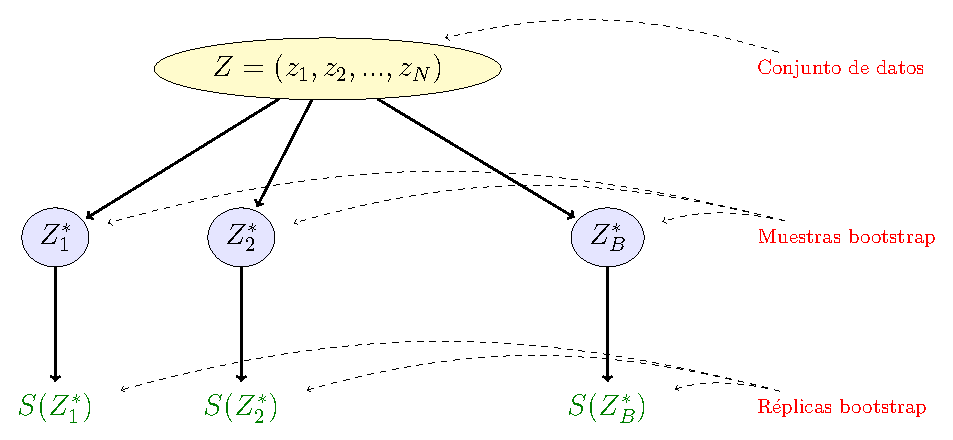
\includegraphics[width=0.9\linewidth]{gfx/bootstrap}}
    \label{fig:bootesq}
  \end{figure}
\end{frame}        

\begin{frame}{Bootsrap paramétrico}
  \begin{itemize} 
    \itemsep1em
    \item El bootstrap clásico es no paramétrico, y se vale únicamente del conjunto observado para a partir de ahí estimar la función de distribución empírica. 

    \item En el caso que nos interesa, se cuenta con un modelo paramétrico que ha sido ajustado a los datos, usualmente por MLE. 

    \item A partir de este modelo ajustado es que se muestrea. Al igual que en con la técnica no paramétrica, se suelen generan muestras de datos del mismo tamaño que el conjunto original. 

    \item Luego, para cada nueva conjunto bootstrap $\mb{Z}^{*}_b$ muestreado se calcula el estadístico de nuestro interés. Éste proceso de muestreo se repite igualmente una gran cantidad de veces. 
  \end{itemize}
\end{frame}

\begin{frame}{Selección de modelo usando BIC}
  \begin{itemize} 
    \itemsep1em

    \item Puesto que consideramos que dentro de nuestro espacio de modelos propuestos se encuentra el modelo solución, resulta más natural usar BIC (cita).

    \item Esta función de penalización se calcula de la siguiente manera: 
    \begin{equation}
    BIC(\mc{M}) = 2 \mc{L}_{max}(\mc{M}) - (log N ) dim(M)
    \end{equation}
    para cada modelo $\mc{M}$, donde $dim(M)$ es el número estimado de parámetros libres que le corresponden, y $N$ es el tamaño de nuestra muestra de datos. 

    \item Por otra parte, $\mc{L}_{max}(\mc{M})$ es la máxima log-verosimilitud obtenida para el modelo $\mc{M}$ después de realizar un número $HMM_{MAX}$ de simulaciones, para evitar que en algún caso el algoritmo de estimación se quede atorado en un máximo local.
  \end{itemize}
\end{frame}


\begin{frame}{Selección de modelo usando BIC}
  \begin{itemize} 
    \itemsep1em

    \item Para estimar el número de parámetros libres de nuestro modelo, se consideran todas las probabilidades que rigen al HMM:
    \begin{itemize} 
      \itemsep0.8em
      \item Matriz a priori o inicial
      \item Matriz de transición entre los interlocutores
      \item Matriz de emisión de cada persona para todo el diccionario de palabras
    \end{itemize}

    \item Este tipo de función de penalización nos permite seleccionar de entre un conjunto de modelos propuestos (que pueden ser muchos) al modelo o los modelos con mayor probabilidad de ser los correctos. 

  \end{itemize}
\end{frame}

\begin{frame}{Selección de modelo usando bootstrap con likelihood ratio testing}
  \begin{itemize} 
    \itemsep1em

    \item Se utilizará la técnica bootstrap paramétrico, pues mediante el algoritmo EM es fácil obtener el modelo parametrizado. 

    \item Usualmente se compararán dos modelos adyacentes, es decir, el modelo $\mc{M}_d$ de $d$ estados contra el modelo $\mc{M}_{d+1}$ de $d+1$ estados ocultos.

    \item Se usa el estadístico LLR que corresponde a la diferencia de las log-verosimilitudes de dos modelos
      \begin{equation}
        LLR^{(d)}_{obs} = \log \frac{L(\hat \theta^{(d+1)}; y_{1:n})}{L(\hat \theta^{(d)}; y_{1:n})} =
          \log L(\hat \theta^{(d+1)}; y_{1:n}) - 
          \log L(\hat \theta^{(d)}; y_{1:n})
      \end{equation}
  \end{itemize}
\end{frame}

\begin{frame}{Selección de modelo usando bootstrap con likelihood ratio testing}
  \begin{itemize} 
    \itemsep1em
    \item Para calcular el MLE de un modelo, se estimó la verosimilitud varias veces con diferentes parámetros iniciales aleatorios. 

    \item Se iteró el algoritmo EM hasta convergencia, un numero $iter_{hmm}$ fijo de iteraciones, esto para evitar el estancamiento del algoritmo en un máximo local, y obtener así una buena estimación de la máxima verosimilitud del modelo.

    \item Se usó entonces como MLE del modelo la máxima verosimilitud correspondiente a los mejores parámetros estimados y que se denotó por $LLR_{obs}$.
  \end{itemize}
\end{frame}


%!TEX root = ../pres - final.tex

\section{Metodología propuesta}

\begin{frame}{Metodología propuesta}
  \begin{figure}[bth]
    \centerline
    {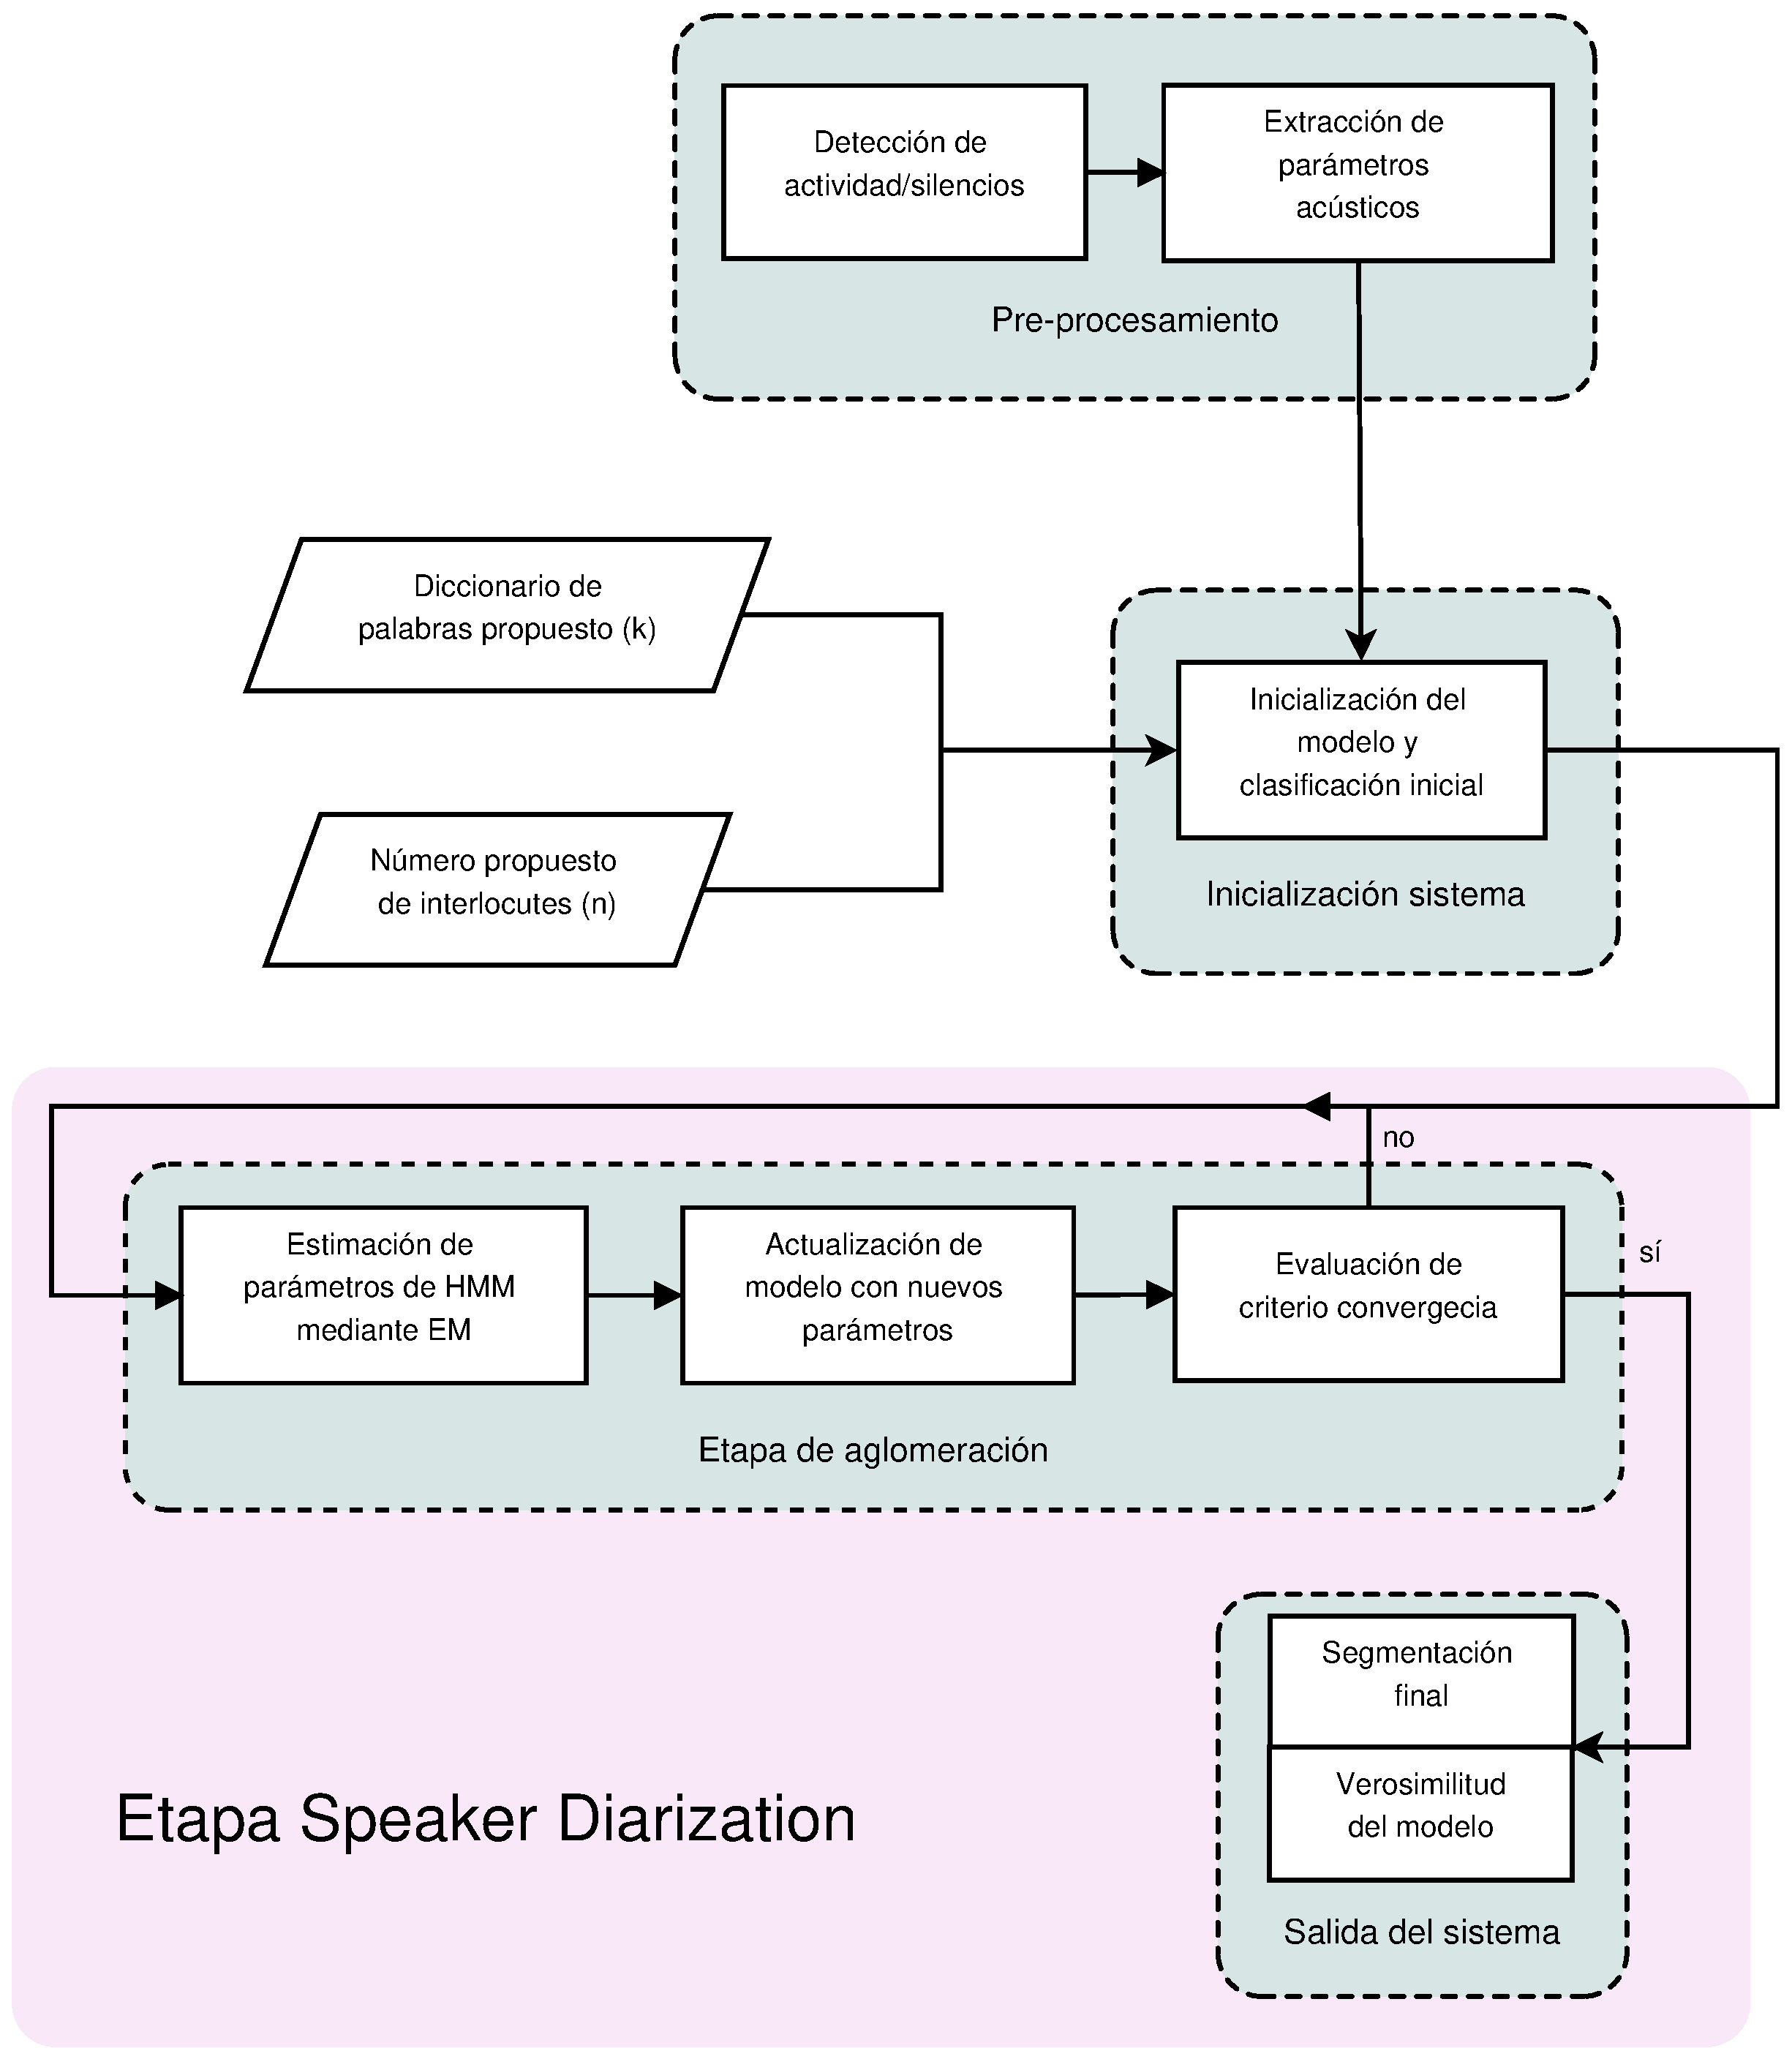
\includegraphics[width=0.6\linewidth]{gfx/general_flow}} \quad
    \caption{Esquema general.}
    \label{fig:esquema}
  \end{figure}
\end{frame}

% \begin{frame}{Selección de modelo realizada}
%   \begin{itemize} 
%     \itemsep1em

%     \item Este proceso se realizara en dos partes: 

%       \begin{itemize} 
%         \itemsep0.8em
%         \item Exploración de todo el espacio de soluciones y reducción de posibles modelos ganadores.
%         \item Selección de mejor modelo entre los candidatos resultantes.
%       \end{itemize}  
%     \end{itemize}   
% \end{frame}

\begin{frame}{Selección de modelo realizada}{Exploración}
  \begin{itemize} 
    \itemsep1em

    \item
    Se estimará BIC de todos los HMM propuestos para generar una curva de selección. 

    \item Como se verá en las pruebas, es necesario introducir un término de regularización en BIC para que la penalización del modelo corresponda con las log-verosimilitudes obtenidas. 
    \begin{equation}
    BIC_{\lambda}(\mc{M}) = 2 \mc{L}_{max}(\mc{M}) - \lambda \cdot log N \cdot dim(M)
    \end{equation}

    \item Se deberá encontrar el valor adecuado para $\lambda$ que penalice de buena forma los modelos. 
    \end{itemize}   
\end{frame}    

\begin{frame}{Selección de modelo realizada}{Exploración}
  \begin{itemize} 
    \itemsep1em
    \item Para escoger el valor adecuado de $\lambda$ se realizará un análisis de sensibilidad, generando múltiples curvas de selección BIC con diferentes valores de $\lambda$. 

    \item Se buscará la región de inflexión que divide a la superficie anterior en dos: en la primera parte de la superficie. 
    %, el valor de $\lambda$ será pequeño, por lo que siempre tendrán una mayor verosimilitud los modelos con más parámetros; mientras que en la segunda parte, la penalización sera muy grande, y se escogerán siempre los modelos más sencillos, sin darle tomar en cuenta su verosimilitud.

    \item Calculando el gradiente de la superficie generada por las funciones BIC, se buscará la región asociada a un $\lambda$ en el que la suma de los valores absolutos sea menor. 

    \item Una vez que se logre seleccionar el $\lambda$ adecuado de regularización, se procede a evaluar su curva BIC asociada y de ahí se obtiene al modelo ganador o un subconjunto de posibles ganadores.
  \end{itemize}   
\end{frame}    

\begin{frame}{Selección de modelo realizada}{Selección}
  \begin{itemize} 
    \itemsep1em

    \item Luego se realizará un proceso de refinamiento en caso de que se tengan varios modelos posibles. 

    \item Se formarán pares de modelos que se deseen comparar, y se estimará su LLR, que se denominará como $LLR_{obs}$. 

    \item Luego, mediante bootstrap paramétrico se hará una prueba de hipótesis para comproar cuál modelo es más adecuado para los datos.

    \item De esta forma, se pueden realizar pruebas de hipótesis para los modelos candidatos, e ir rechazando modelos de acuerdo al análisis propuesto. 

  \end{itemize}   
\end{frame}    



%!TEX root = ../pres - final.tex

\section{Pruebas y resultados}

\subsection{Pruebas}

\begin{frame}{Secuencia 3}{Parámetros}

\begin{figure}[t!]
  \centerline{  
    \hspace{1.2cm}
    \parbox[c]{0.22\textwidth}{\centering Modelo generador}
    \parbox[c]{0.22\textwidth}{\centering Modelo $n_3$}
    \parbox[c]{0.22\textwidth}{\centering Modelo $n_4$}
    \parbox[c]{0.22\textwidth}{\centering Modelo $n_5$}
  }
  \vspace{0.5cm}
  \foreach \row in {1, ..., 2}{%  
    \centerline{%
      \parbox[c]{0.5cm}{
        \vspace{0cm}
        \myheader{\row}
      }
      %\gdef \widthimg {0.35}
      \foreach \col in {1, ..., 4}{%
        \pgfmathparse{\col == 4 && \row == 2? 1:0}
        \ifthenelse{\pgfmathresult=1}{
          \gdef \widthimg {0.22}
        }{
          \gdef \widthimg {0.18}
        }
        \begin{subfigure}[c]{\widthimg \textwidth}          
          \def \imgfile {gfx/chap6/lear3p_\col_\row}
          \IfFileExists{\imgfile.eps}{
            \includegraphics[width=1\textwidth]{\imgfile}
            \label{fig:seq1p_\col_\row}
          }{
            \hspace{1\textwidth}
          }
        \end{subfigure}
        %\hspace{-0.005\textwidth}
      }
    }
  }
\label{fig:seq1p}
\end{figure}

\end{frame}

\begin{frame}{Secuencia 3}{Parámetros}
  \begin{figure}[tp]
    \centerline{
      \hspace{1cm}
      \parbox[c]{0.22\textwidth}{\centering Modelo generador}
      \parbox[c]{0.18\textwidth}{\centering Modelo $n_3$}
      \parbox[c]{0.18\textwidth}{\centering Modelo $n_4$}
      \parbox[c]{0.18\textwidth}{\centering Modelo $n_5$}
    }
    \vspace{0.5cm}
    \foreach \row in {3, ..., 7}{%  
      \centerline{
        \parbox[c]{1cm}{
          \vspace{-0.3cm}
          \myheader{\row}
        }
        \foreach \col in {1, ..., 4}{%
          \begin{subfigure}[c]{0.18\textwidth}  
            \def \imgfile {gfx/chap6/lear3p_\col_\row}
            \IfFileExists{\imgfile.eps}{
              \includegraphics[width=1\textwidth]{\imgfile}
              \label{fig:seq1p_\col_\row}
            }{
              \hspace{1\textwidth}
            }
          \end{subfigure}
        }
      }
    }  
  \label{fig:seq1q}
  \end{figure}
  
\end{frame}

\begin{frame}{Secuencia 3}{Superficie BIC}
\begin{figure}[t!]
  \centerline{
  \begin{subfigure}[b]{0.7\textwidth}
   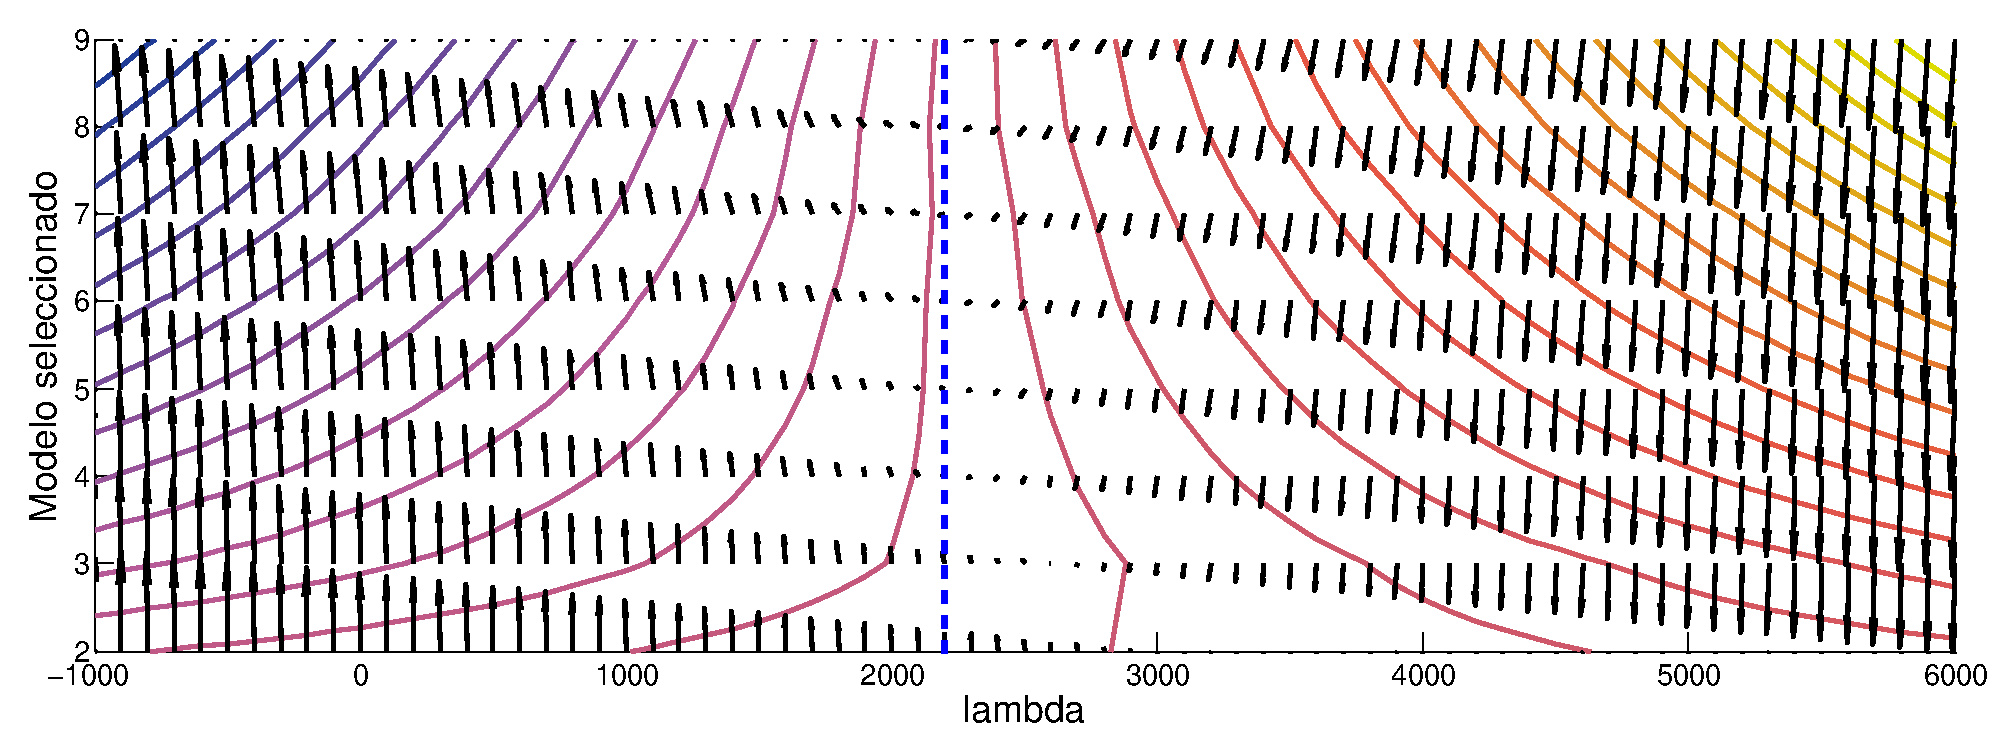
\includegraphics[width=1\textwidth]{gfx/chap6/lear3bic2}
   \caption{}
   \label{fig:seq3_bic2}
  \end{subfigure}  
  }  
  \centerline{
  \begin{subfigure}[b]{0.4\textwidth}
    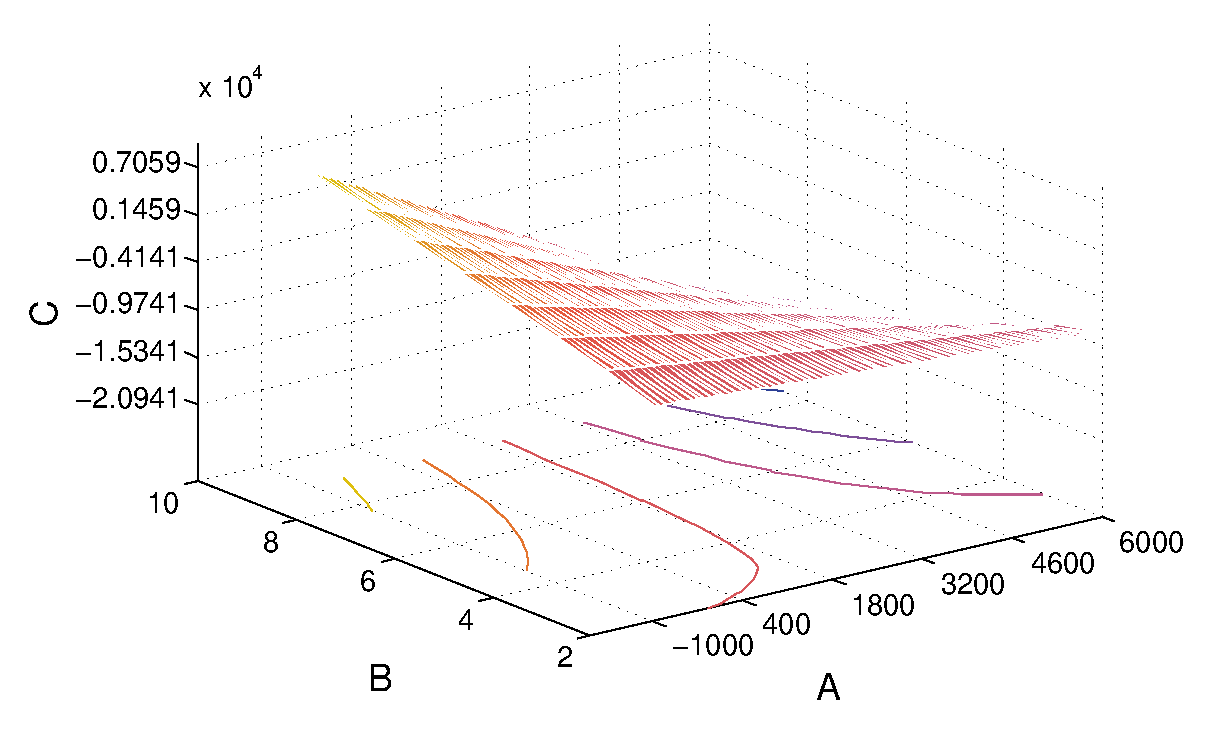
\includegraphics[width=\textwidth]{gfx/chap6/lear3bic1} 
    \caption{}
    \label{fig:seq3_bic1}
  \end{subfigure}  
  \begin{subfigure}[b]{0.4\textwidth}
    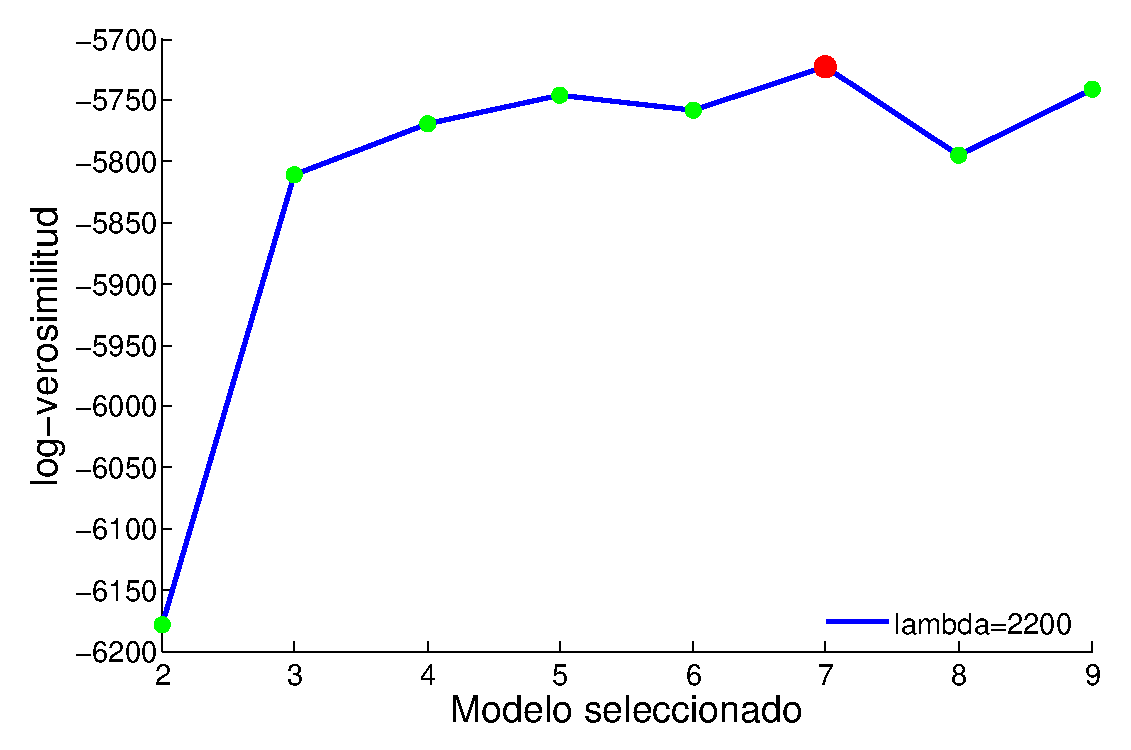
\includegraphics[width=\textwidth]{gfx/chap6/lear3bic3} 
    \caption{}
    \label{fig:seq3_bic3}
  \end{subfigure}
  }
  \label{fig:seq1_bic}
\end{figure}
\end{frame}

\begin{frame}{Secuencia 3}{Pruebas de hipótesis}
\begin{figure}[t!]
  \centerline  
  { \begin{subfigure}[b]{0.45\textwidth}
      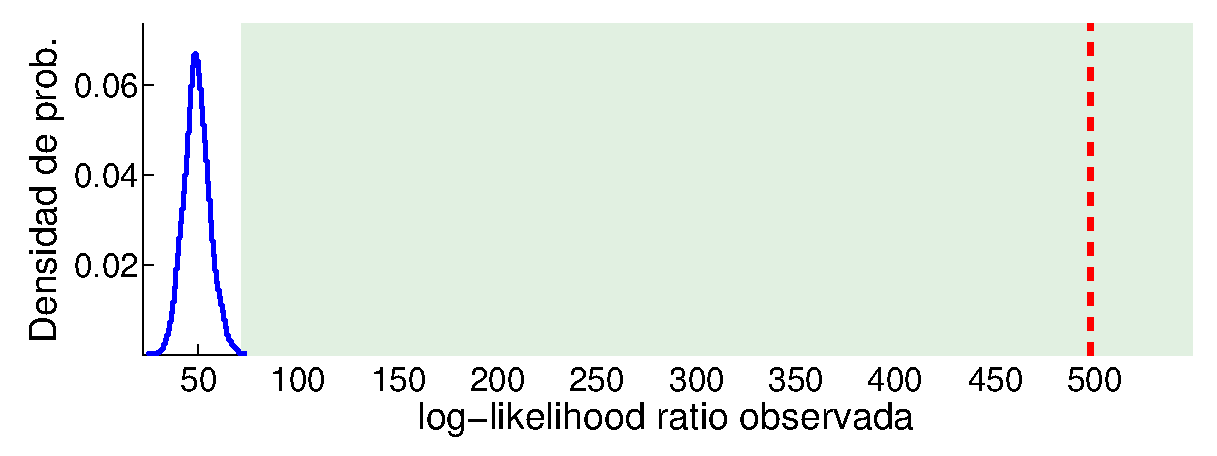
\includegraphics[width=1\linewidth]{gfx/chap6/lear3boot1}
      \caption{}
      \label{fig:seq3_boot1}
    \end{subfigure}
    \hspace{0.5cm}
    \begin{subfigure}[b]{0.45\textwidth}
      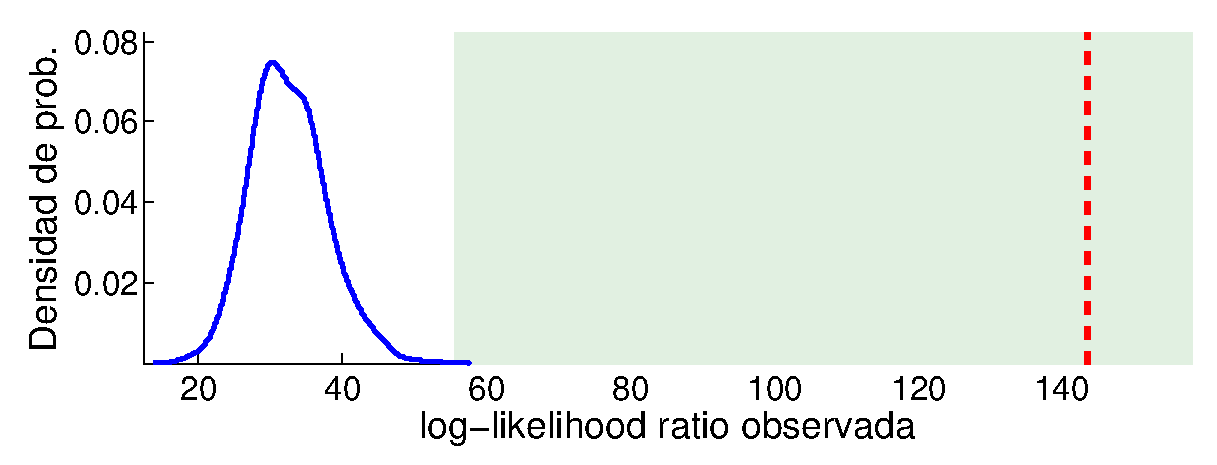
\includegraphics[width=1\linewidth]{gfx/chap6/lear3boot2}
      \caption{}
      \label{fig:seq3_boot2}
    \end{subfigure}
  }
  \centerline  
  { \begin{subfigure}[b]{0.45\textwidth}
      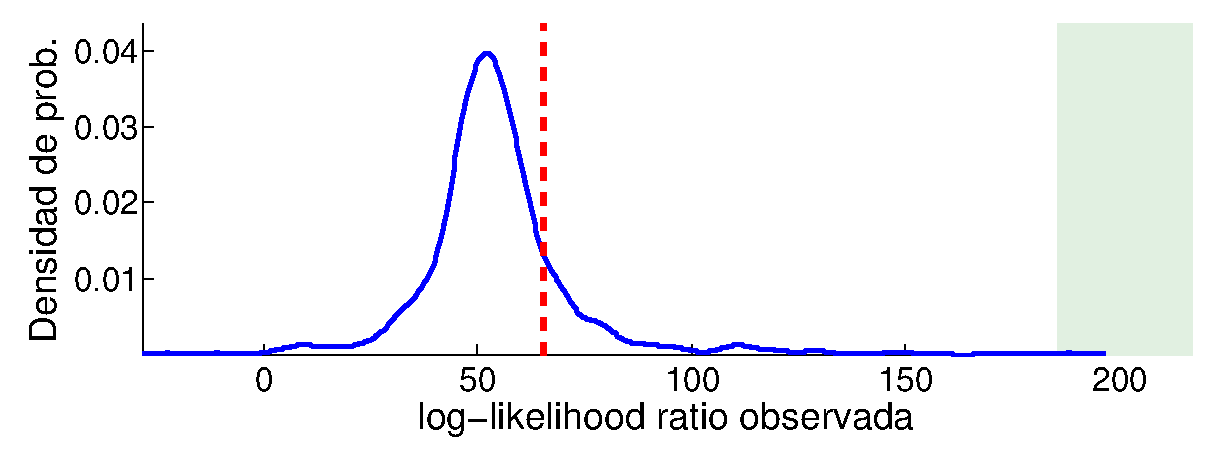
\includegraphics[width=1\linewidth]{gfx/chap6/lear3boot3}
      \caption{}
      \label{fig:seq3_boot3}
    \end{subfigure}
    \hspace{0.5cm}
    \begin{subfigure}[b]{0.45\textwidth}
      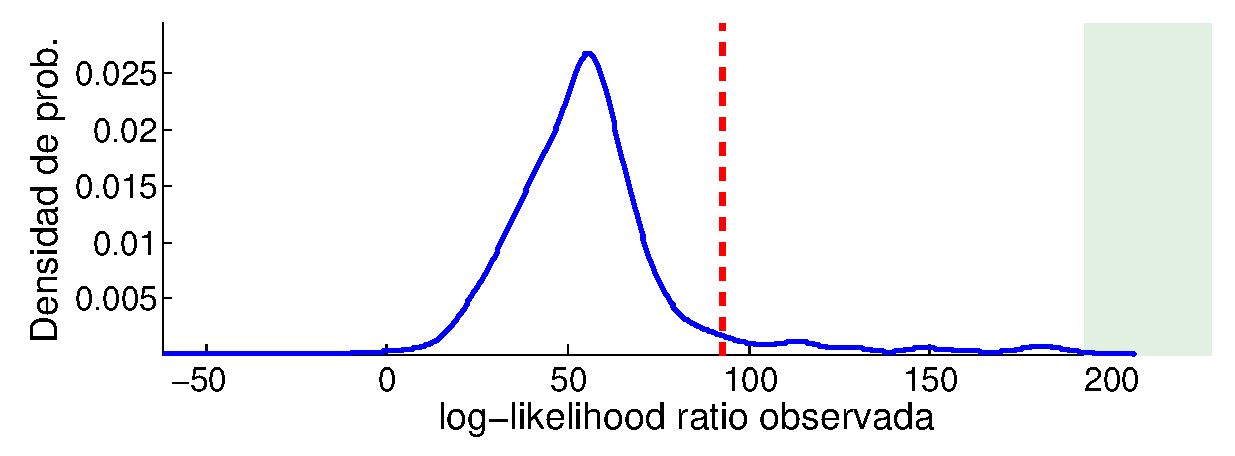
\includegraphics[width=1\linewidth]{gfx/chap6/lear3boot4}
      \caption{}
      \label{fig:seq3_boot4}
    \end{subfigure}
  }
  \label{fig:seq3_boot}
\end{figure}
\end{frame}

\begin{frame}{Secuencia 3}{Secuencia recuperada}
\begin{figure}[tp]
  \centerline
  {\begin{subfigure}[b]{0.8\textwidth}
      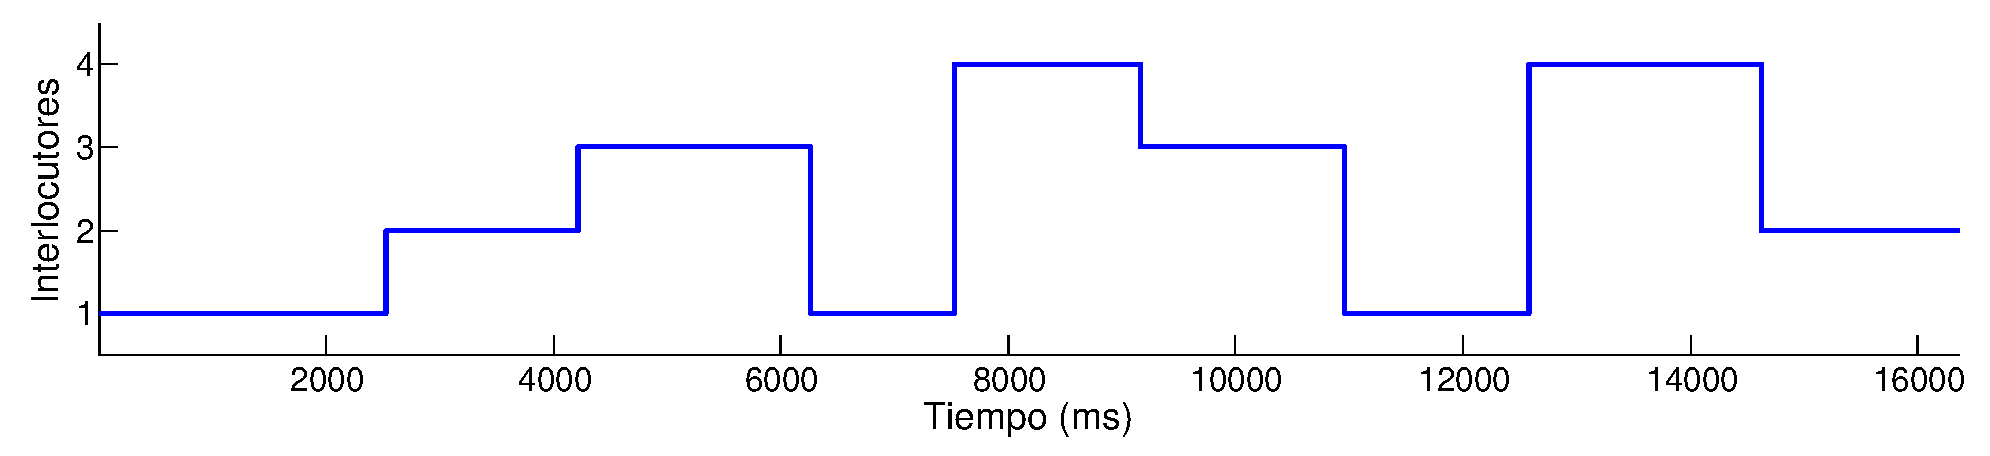
\includegraphics[width=1\linewidth]{gfx/chap6/lear3s_3_1}
      \caption{}
      \label{fig:seq3_seq1}
    \end{subfigure}
  } 
  \centerline
  {\begin{subfigure}[b]{0.8\textwidth}
      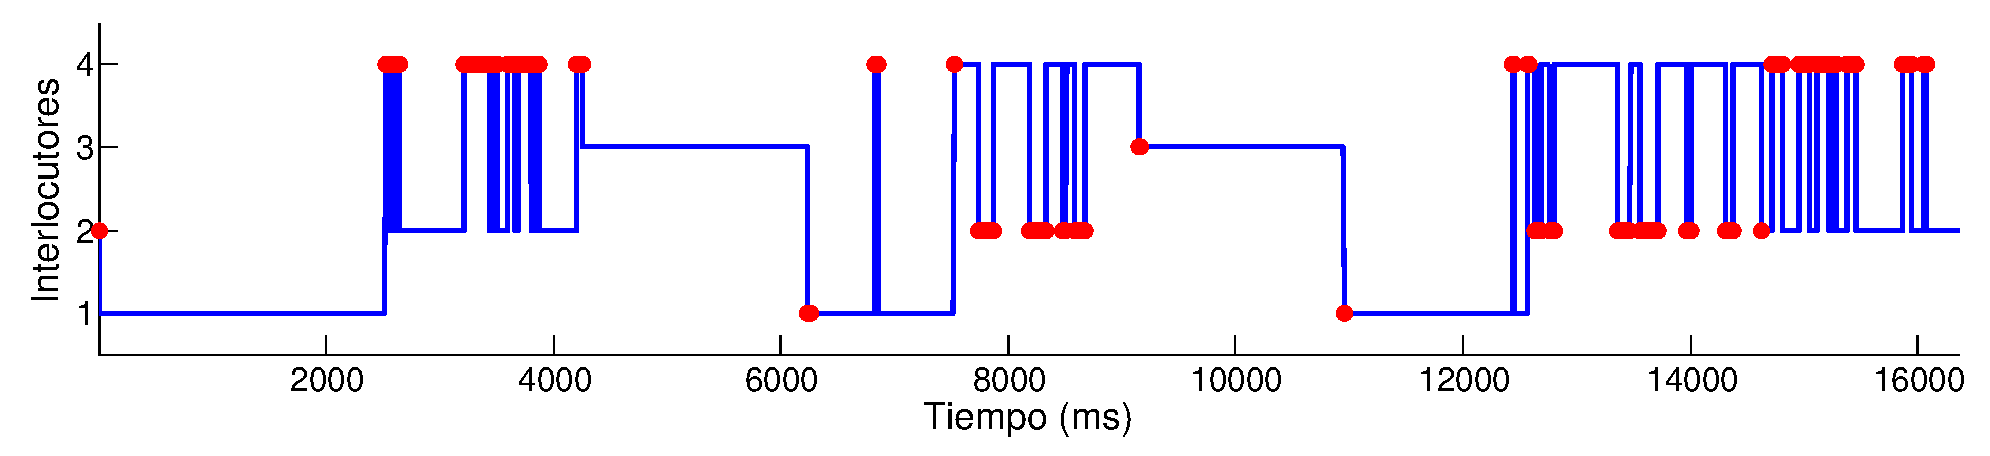
\includegraphics[width=1\linewidth]{gfx/chap6/lear3s_3_2}
      \caption{}
      \label{fig:seq3_seq2}
    \end{subfigure}
  }
  \label{fig:prb3_seq}
\end{figure}
\end{frame}

\subsection{Resultados}
\begin{frame}{Tabla de resultados (I)}
  Descripción de las secuencias de audio utilizadas para las pruebas.
  \begin{figure}[bth]
    \centerline
    {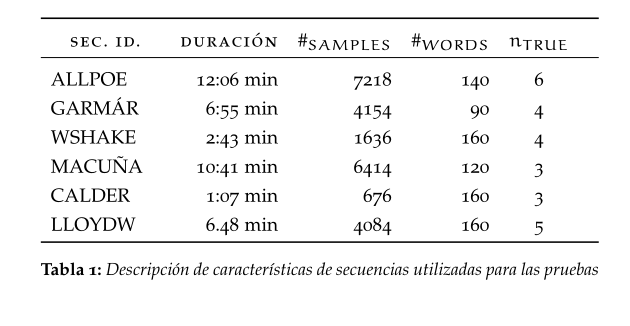
\includegraphics[width=0.7\linewidth]{gfx/tab1}}
    \label{fig:esquema}
  \end{figure}  
\end{frame}

\begin{frame}{Tabla de resultados (II)}
  Detalle de los resultados para todas las secuencias de audio.
  \begin{figure}[bth]
    \centerline
    {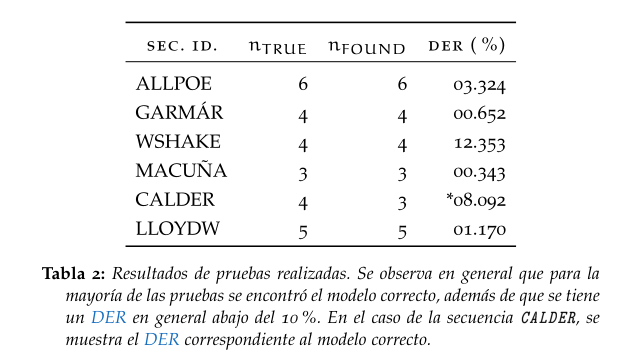
\includegraphics[width=0.7\linewidth]{gfx/tab2}}
    \label{fig:esquema}
  \end{figure}  
\end{frame}

%!TEX root = ../pres - final.tex

\section{Conclusiones}

\begin{frame}{Conclusiones}
  \begin{enumerate}
    \itemsep0.8em
    \item De acuerdo a los resultados obtenidos, se observa que el método presentado muestra un buen desempeño en las pruebas realizadas. 

    \item La metodología propuesta permite una rápida exploración de todos los modelos propuestos, así como una selección del mejor candidato de acuerdo a las pruebas de hipótesis que se plantean.

    \item La calidad de los resultados depende en gran parte de un correcto pre-procesamiento de la señal; ya sea para eliminar ruidos, así como para la correcta parametrización de los vectores característicos.

    \item Aunque el método presentado realiza pruebas computacionalmente intensivas, desde la primera etapa de exploración permite identificar a un sub-conjunto pequeño de posibles modelos correctos.

    \item La importancia de la segunda etapa de selección, permite dar certeza sobre cuál de los modelos es el correcto. Incluso con un alto nivel significancia, las pruebas de hipótesis suelen seleccionar de buena forma al modelo ganador.
  \end{enumerate}
\end{frame}

\begin{frame}{Trabajo futuro}
\begin{enumerate}
    \itemsep0.8em

    \item Construir un banco de pruebas con voces reales, que permitan analizar el comportamiento del método presentado en un entorno más real.

    \item Mejorar la forma en que se eliminan los silencios y ruidos; pues en pruebas con un ambiente \textit{normal}, hay muchas más fuentes de perturbación que las que hasta ahora se han considerado. 

    \item Explorar otras estrategias para selección de la segmentación más óptima, buscando realizar el cálculo de manera eficiente.

    \item Evaluar la pertinencia de paralelizar el algoritmo principal de estimación de parámetros del HMM, para mejorar el rendimiento general del sistema.
\end{enumerate}
\end{frame}

% All of the following is optional and typically not needed. 
\appendix
\section<presentation>*{\appendixname}
\subsection<presentation>*{Referencias}

\begin{frame}[allowframebreaks]
  \frametitle<presentation>{Referencias}
    
  \begin{thebibliography}{10}
    
  \beamertemplatebookbibitems

  \bibitem{Author1990}
    A.~Author.
    \newblock {\em Handbook of Everything}.
    \newblock Some Press, 1990.
 
    
  \beamertemplatearticlebibitems

  \bibitem{Someone2000}
    S.~Someone.
    \newblock On this and that.
    \newblock {\em Journal of This and That}, 2(1):50--100,
    2000.
  \end{thebibliography}
\end{frame}

\end{document}